\chapter{Энергонезависимая память на основе сегнетоэлектрических материалов}\label{ch:ch1}
При проведении исследований по разработке устройств памяти на основе новых физических принципов важно понимать текущее состояние технологий, используемых в производстве: принципы работы устройств, их характеристики, преимущества и возможности по их дальнейшему улучшению. Это позволяет критически оценивать уровень полученных разработок, а также понимать какими характеристиками должны обладать устройства на новых физических принципах для их внедрения в производство.
\section{Флеш-память}\label{sec:ch1/sec1}
На момент написания этой работы доминирующим на рынке видом энергонезависимой памяти (NVM) является флеш-память. Основным компонентом флеш-памяти является транзистор с плавающим затвором (рис. \cref{fig:floating_gate_transistor}). При приложении потенциала к управляющему затвору происходит туннелирование электронов сквозь диэлектрической слой, что приводит к инжекции заряда в плавающий затвор и обеспечивает запись информации в устройстве. При считывании прикладывается напряжение между стоком и истоком, проводимость канала транзистора при этом определяется наличием заряда на плавающем затворе: в отсутствии заряда ток протекает, а при наличии заряда канал остаётся закрытым.

При отсутствии напряжения на плавающем затворе ток через диэлектрик значительно уменьшается, тем самым обеспечивая длительное хранение заряда в затворе, а значит и долгий срок хранения информации в устройстве.

\begin{figure}[ht]
    \centerfloat{
        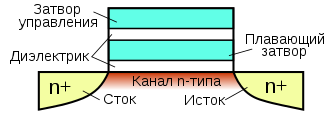
\includegraphics[scale=0.8]{floating_gate_transistor.png}
    }
    \caption{Транзистор с плавающим затвором}\label{fig:floating_gate_transistor}
\end{figure}

Стоит отметить, что в большинстве современных устройств флеш-памяти используются многобитовые ячейки памяти (multi-level cell), которые позволяют увеличить объём хранимой информации за счёт увеличения количества различимых состояний заряда на затворе (\(2^N\) состояний соответствуют \(N\) битам памяти).

Кроме того, для повышения объёма записи в данный момент используется увеличение количества слоёв с ячейками памяти в чипе (3D NAND), а также технология трёхмерной интегральной микросхемы (3D IC), позволяющая упаковывать несколько чипов в одном устройстве.

\section{Сегнетоэлектрическая память}\label{sec:ch1/sec2}
\todo{добавь, зачем заменять флеш, неубедительно, характеристики растут}

\noindent По сравнению с флеш-памятью, сегнетоэлектрическая память обладает рядом потенциальных преимуществ:
\begin{itemize}
    \item Более низкое энергопотребление при записи.
    \item Более высокая скорость записи.
    \item Большее количество циклов перезаписи.
    \item Возможность создания <<универсальной>> памяти, сочетающей в себе скорость работы памяти с произвольным доступом (DRAM) и энергонезависимость.
\end{itemize}

\todo{В связи с этим ведутся разработки бла-бла, мб упомянуть ReRAM, MRAM, etc., если в тему будет, мб section переименовать}
\subsection{Сегнетоэлектрики}
Сегнетоэлектричество (СЭ) "--- свойство материалов, позволяющее им обладать спонтанной поляризацией. То есть в отсутствии внешнего электрического поля в таких веществах сохраняется ненулевой вектор поляризации. Наличие этого свойства в материале определяется кристаллической решёткой. Так, СЭ может проявляться лишь в таких пространственных группах (фазах) вещества, кристаллическая решётка (сингония) которых не является центросимметричной.

Одним из наиболее характерных свойств СЭ материалов является наличие петли гистерезиса в зависимости поляризации \(P\) от напряжённости электрического поля \(E\) (рис. \cref{fig:hysteresis}). Важные характеристики, которые часто используются при характеризации СЭ материалов: коэрцитивное поле и остаточная поляризация также отражены на рисунке \cref{fig:hysteresis}. Стоит отметить, что зависимость такого вида может быть получена и в несегнетоэлектрических материалах за счёт зарядки/разрядки ловушек в диэлектрике, а значит не может быть использована как критерий проявления СЭ в материалах.

\begin{figure}[ht]
    \centerfloat{
        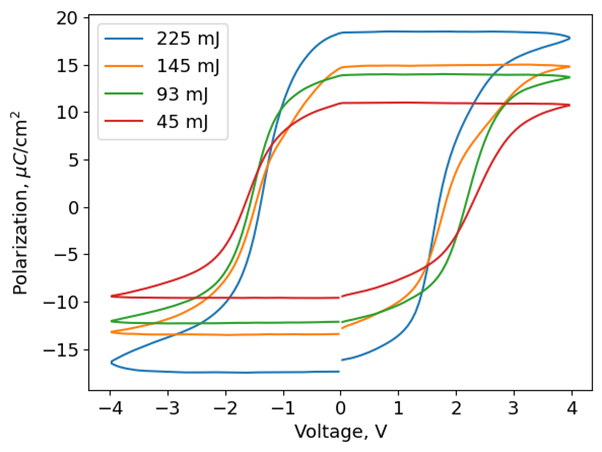
\includegraphics[scale=0.8]{hysteresis.png}
    }
    \caption{Зависимость поляризации \(P\) от напряжённости электрического поля \(E\) в сегнетоэлектрике}\label{fig:hysteresis}
\end{figure}

\todo{уже была секция сегнетоэлектрики, подумай над структурой}
\subsubsection{Перовскитоподобные материалы/материалы перовскитной структуры}
Классическими материалами, обладающими СЭ свойствами являются перовскитоподобные материалы вида ABO\(_3\), в частности Pb[Zr\(_x\)Ti\(_{1-x}\)]O\(_3\) (PZT) (рис. \cref{fig:pzt})
\todo{не совместимы с КМОП, т.к. требуют применения электродов на основе материалов из благородных металлов}
\begin{figure}[ht]
    \centerfloat{
        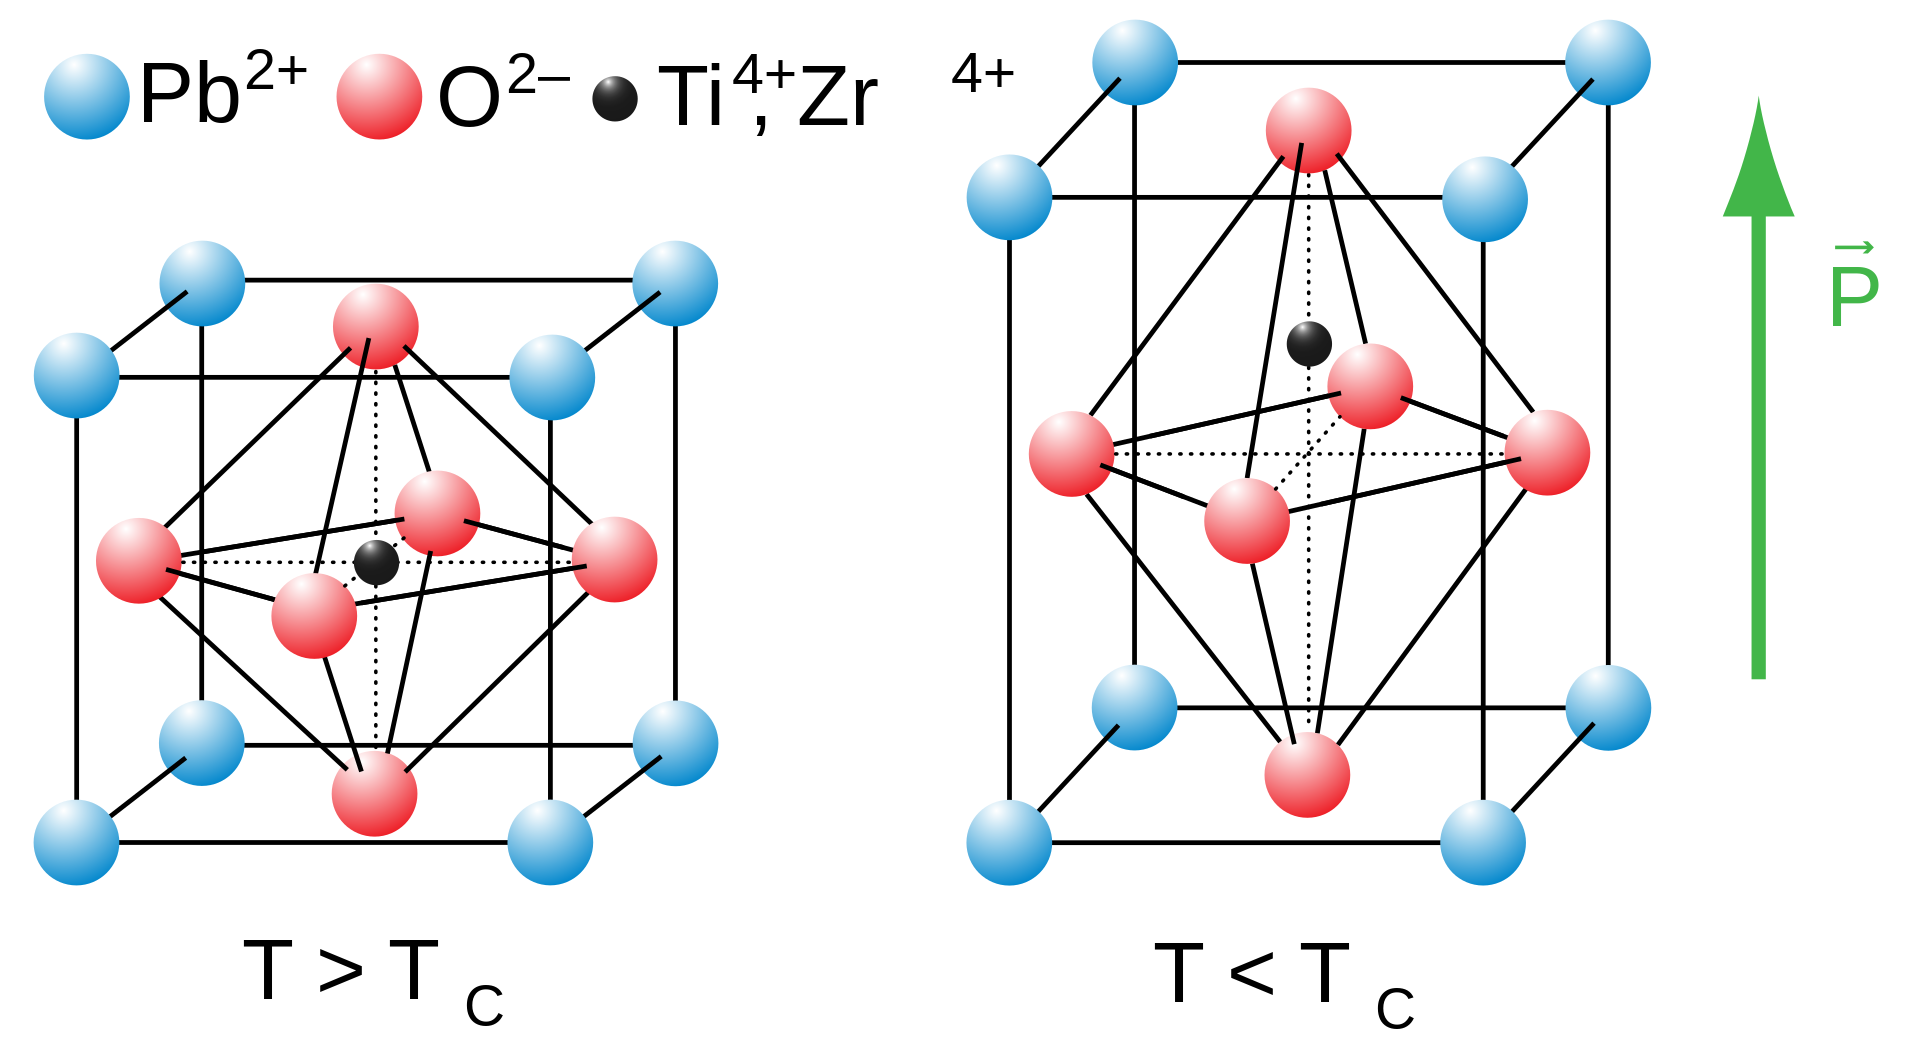
\includegraphics[width=0.8\linewidth]{pzt.png}
    }
    \caption{Кристаллическая структура PZT при температурах выше и ниже точки Кюри \(T_c\)}\label{fig:pzt}
\end{figure}

Необходимость создания слоёв с толщиной СЭ слоя \(~\) \SI{70}{\nano\meter} существенно ограничивает возможность масштабирования устройств на основе перовскитных материалов \cite{parkReviewPerspectiveFerroelectric2018}. Уменьшение толщины приводит к возрастанию тока утечек, что приводит к невозможности достоверного считывания состояния ячейки.
\subsubsection{Сегнетоэлектрический оксид гафния}\label{sec:ch2/sec1}
Более перспективным и интересным для исследования материалом является оксид гафния HfO\(_2\). В 2007 было сообщено об использовании данного материала (наряду с ZrO\(_2\)) в качестве подзатворного диэлектрика в полевом транзисторе для уменьшения токов утечки через подзатворный слой \cite{bohrHighkSolution2007}. В 2011 году в оксиде гафния были обнаружены СЭ свойства \cite{bosckeFerroelectricityHafniumOxide2011}.

При нормальных условиях в оксиде гафния энергетически выгодной является неполярная моноклинная фаза \(P2_1/c\). %, неполярная орторомбическая \(Pbca\), полярная орторомбическая \(Pca2_1\).
Однако, при определённых условиях возможна стабилизация полярной (сегнетоэлектрической) орторомбической фазы \(Pca2_1\). СЭ свойства при этом определяются отсутствием центральной симметрии в кристаллической решётке.
Было показано, что за снижение свободной энергии СЭ фазы и её стабилизацию в оксиде гафния отвечает ряд характеристик. Так, необходим существенный вклад поверхностной энергии в свободную энергию, который достигается при достаточном уменьшении толщины плёнки. Кроме того, значительным фактором, влияющим на стабилизацию фазы, являются механические напряжения в оксиде гафния. Известно, что в отсутствии верхнего электрода СЭ свойства структур на основе оксида гафния значительно ухудшаются. Этот эффект объясняется тем, что при быстрой термической обработке структуры с нижним и верхним электродами, в оксиде гафния возникают механические напряжения, которые образуются за счёт различия в коэффициенте теплового расширения материалов электродов и оксида гафния и приводят к образованию орторомбической фазы за счёт подавления образования моноклинной фазы. Наконец, важнейшим элементом является легирование оксида. СЭ свойства разной степени выраженности были получены в плёнках с примесями Si \cite{bosckeFerroelectricityHafniumOxide2011}, Zr \cite{bosckePhaseTransitionsFerroelectric2011}, La \cite{schroederLanthanumDopedHafniumOxide2018}, Al \cite{muellerIncipientFerroelectricityDoped2012}, Gd \cite{}, Y \cite{}, Ga \cite{chouprikNanoscaleDopingIts2022}. Несмотря на широкий спектр возможностей по выбору примесного элемента, использование большинства из указанных элементов приводит к повышению температуры кристаллизации плёнки значительно выше 400 \si{\degreeCelsius}, тем самым нарушая возможную совместимость с backend-of-line (BEOL) процессом в CMOS технологии \cite{schmitzLowTemperatureThin2018}, существенно затрудняя внедрение устройств памяти на основе оксида гафния в производство. Одним из наиболее перспективных материалов для создания энергонезависимой памяти является твёрдый раствор Hf0.5Zr0.5O2. Обладая сравнительно невысокой температурой кристаллизации \(\approx\) \SI{400}{\degreeCelsius}, и одинаковой долей элементов Hf и Zr, позволяющей контролировать стехиометрию с большой точностью, HZO ... структуры на основе имеют ... остаточной поляризации (или не надо про это пока)

\subsection{Устройства памяти на основе сегнетоэлектриков}
Наличие двух стабильных состояний кристаллической решётки, которым соответствует положительная и отрицательная поляризация материала \todo{(рис. со свободной энергией} позволяет использовать СЭ материалы как функциональный слой в устройствах энергонезависимой памяти. При этом запись осуществляется приложением электрического поля к СЭ слою, а чтение может быть осуществлено различными способами. Основные концепции сегнетоэлектрической памяти включают в себя коммерчески доступную сегнетоэлектрическую память с произвольным доступом (ferroelectric random access memory, FeRAM), сегнетоэлектрический полевой транзистор (ferroelectric field-effect transistor, FeFET) и сегнетоэлектрический туннельный переход (ferroelectric tunnel junction, FTJ), принципиальные схемы которых отражены на рисунке \cref{fig:FeRAM}. \todo{Мб добавить описание принципов считывания, поясняющее картинку}
\todo{Не знаю куда вставить
    К основным недостаткам FeRAM можно отнести низкую плотность записи, по причине необходимости создания структур один транзистор -- один конденсатор (1T-1C); невозможность хранения более одного бита в ячейке, поскольку вектор поляризации, напрямую определяющий значение бита, может находиться лишь в двух состояниях; а также деструктивность считывания.}

\begin{figure}[ht]
    \centerfloat{
        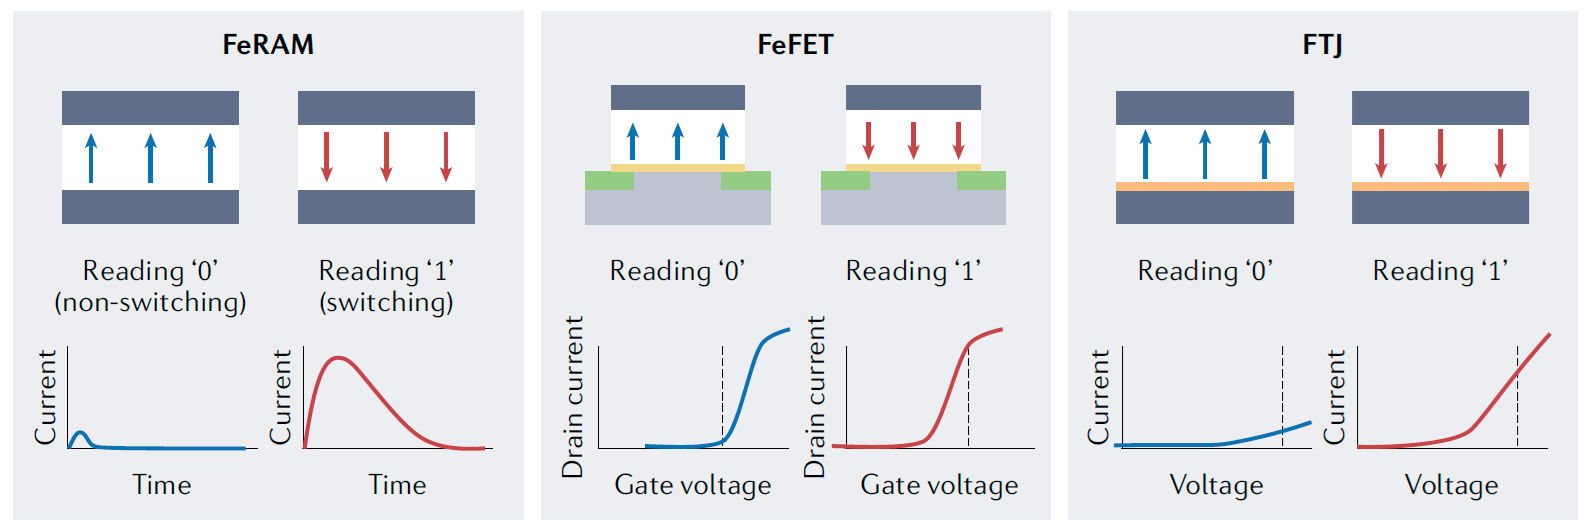
\includegraphics[scale=0.5]{FeRAM.png}
    }
    \caption{Схемы концепций сегнетоэлектрической памяти \cite{schroederFundamentalsApplicationsFerroelectric2022}}\label{fig:FeRAM}
\end{figure}

\FloatBarrier
